% ====================================================================================================
% SECTION 5  RESULTS  (budget ~2.8 pages)
%   5.1 RQ1 agreement (Table 3, Figure 3) | 5.2 RQ2a error sensitivity (Table 4) | 5.3 RQ2b what limits reliability
% ====================================================================================================

\section{Results}
\label{sec:results}

\subsection{RQ1: Does the score track true quality?}
\label{sec:rq1}

\begin{table*}[t]
  \centering
  \small
  \setlength{\tabcolsep}{5pt}
  \fitbox{\begin{tabular}{@{}lcccccc@{}}
    \toprule
    & \multicolumn{5}{c}{Flat text} & Paragraphs given \\
    \cmidrule(lr){2-6}\cmidrule(l){7-7}
    Evaluator & EWT dev & LinES tr+dev & GENTLE & EWT test & LinES test & EWT dev \\
    & (T) & (T) & (R) & (R) & (R) & (T) \\
    \midrule
    B1 punctuation rule & 0.378 & 0.296 & 0.383 & 0.369 & 0.437 & 0.796 \\
    B3 masked LM (PuncEv) & 0.464 & 0.440 & 0.542 & 0.508 & 0.758 & 0.698 \\
    B8 GPT-2 perplexity & 0.062 & 0.049 & 0.064 & 0.043 & $-$0.322 & 0.039 \\
    B6 consensus & 0.657 & 0.468 & 0.830 & 0.657 & 0.861 & 0.625 \\
    B9 Dawid--Skene & 0.615 & 0.480 & 0.838 & 0.655 & 0.859 & 0.609 \\
    B4 SaT-12l-sm as reference & 0.738 & \textbf{0.630} & 0.880 & 0.754 & \textbf{0.888} & 0.797 \\
    B5 SaT-12l-sm probabilities & 0.762 & \textbf{0.630} & 0.891 & \textbf{0.778} & 0.873 & 0.835 \\
    \midrule
    Ours & \textbf{0.797} & 0.563 & \textbf{0.907} & \textbf{0.787} & 0.873 & \textbf{0.851} \\
    \bottomrule
  \end{tabular}}
  \caption{V1: global Spearman $\rho$ between score and true F1 over all items (Eq.~\ref{eq:rho}). \textbf{Bold}: best in
  the column and values within 0.01 of it. B3, B5 and B9 use our
  scoring $\Qt$ on their own probabilities; B4 and B6 compute F1 against a pseudo-reference. Status letters refer to
  our evaluator; all baseline rows are post hoc (P). B2 length prior and B7 DocAgree, GUM (D), and all CIs and paired
  differences are in App.~\ref{app:agreement}.}
  \label{tab:agreement}
\end{table*}

\begin{figure*}[t]
  \centering
  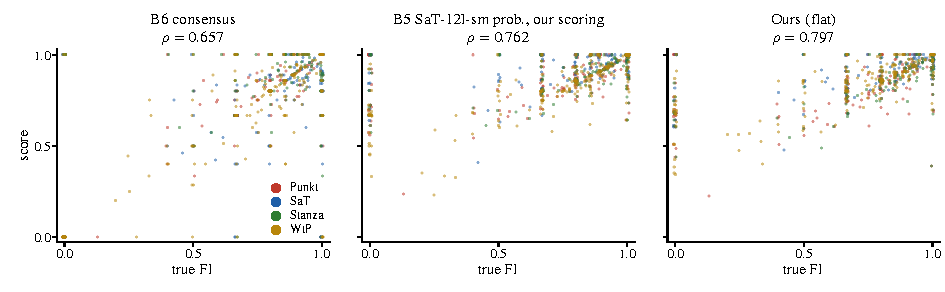
\includegraphics[width=\textwidth]{figures/f3_scatter.pdf}
  \caption{Score vs.\ true F1 for all 1{,}272 items of EWT dev (flat text, T for ours), colored by segmenter. Consensus
  takes few distinct values and gives full marks to many imperfect outputs. The column at true F1 $= 0$ (66 items) holds
  short documents in which a single boundary error drives F1 to 0, e.g., 32 single-sentence documents that a segmenter
  split; every evaluator scores many of them highly.}
  \label{fig:scatter}
\end{figure*}

Table~\ref{tab:agreement} and Figure~\ref{fig:scatter} show agreement with true quality. On the fresh EWT dev split our
evaluator reaches $\rho = 0.797$ on plain text. The paired differences (ours minus baseline, 95\% CI) are large against everything that
does not use a strong supervised segmenter: consensus $+0.141$ [$+0.075$, $+0.213$], Dawid--Skene $+0.183$ [$+0.117$,
$+0.253$], masked LM $+0.333$ [$+0.256$, $+0.414$], the punctuation rule $+0.419$ [$+0.334$, $+0.503$] and GPT-2
$+0.735$ [$+0.640$, $+0.838$]. Given paragraphs, our evaluator beats consensus by $+0.227$ [$+0.158$, $+0.298$]---the
pre-registered primary test---and the rule by $+0.055$ [$+0.033$, $+0.083$]; the rule becomes strong (0.796) once
paragraph breaks are given, because most unpunctuated boundaries in EWT are paragraph breaks. On GENTLE the gain over
consensus is $+0.077$ [$+0.021$, $+0.141$]. LinES is different: on train+dev ours beats consensus only narrowly ($+0.095$
[$+0.007$, $+0.210$]) and the masked LM not significantly ($+0.124$ [$-0.061$, $+0.369$]); on LinES test the gain over
consensus is $+0.011$ (n.s.). GPT-2 perplexity is a useful contrast: it separates candidates within a document (pairwise
accuracy 0.71 on EWT dev) but not across documents, because its likelihood mostly reflects what a document is about---the
confound that normalization removes from Soft F1.

\paragraph{Against a strong segmenter.} Our evaluator is not significantly different from SaT-12l-sm's probabilities in
our scoring on any held-out split: EWT dev $+0.035$ [$-0.014$, $+0.088$], GENTLE $+0.015$ [$-0.035$, $+0.064$], LinES
train+dev $-0.066$ [$-0.236$, $+0.095$], where SaT is ahead (0.630 vs.\ 0.563). It is better than SaT's own segmentation
used as a reference on web text (EWT dev $+0.060$ [$+0.008$, $+0.112$]) but not elsewhere. So evidence that combines
course techniques with pretrained models is statistically indistinguishable from the best supervised segmenter used as
an evaluator; we show next that the
two fail on different errors. An unweighted average of the two is best on web text (EWT dev 0.808, $+0.046$
[$+0.003$, $+0.092$] over B5) but not on LinES (App.~\ref{app:agreement}).

\paragraph{Ranking the segmenters (V2).} Given paragraphs, ours and B5 rank the four segmenters perfectly in every EWT dev
genre (genre-mean $\tau = 1.0$), whereas consensus does not (0.47): it rewards the segmenter that agrees with the
majority, not the one that is right. On flat text the genre-level ranking is noisy for all evaluators (five genres;
ours 0.53, B5 0.67, consensus 0.60), while the document-level $\tau$ favors ours (0.70 vs.\ 0.52 for consensus).
SaT-based evaluators slightly overrate the SaT candidate (rank residual $+0.02$ to $+0.03$), a mild form of the
same-family bias of \citet{deutsch-etal-2022-limitations} (App.~\ref{app:agreement}).

Spearman correlation tells how well a score tracks quality overall. Which errors does it actually notice?

\subsection{RQ2a: Which errors does each evaluator notice?}
\label{sec:rq2a}

\begin{table}[t]
  \centering
  \small
  \setlength{\tabcolsep}{2.6pt}
  \fitbox{\begin{tabular}{@{}lcccccc@{}}
    \toprule
    & \multicolumn{3}{c}{Missed boundary} & \multicolumn{2}{c}{False split} & \\
    \cmidrule(lr){2-4}\cmidrule(lr){5-6}
    Evaluator & term. & par. & in-par. & abbr. & punct. & Ctrl. \\
    \midrule
    B1 rule & \textbf{1.00}\sig & 0.01 & 0.01 & 0.00 & \textbf{0.97}\sig & 0.50 \\
    B8 GPT-2 & 0.82\sig & 0.86\sig & \textbf{0.89}\sig & 0.53 & 0.87\sig & 0.49 \\
    B6 consensus & \textbf{1.00}\sig & 0.52 & 0.51 & 0.55 & \textbf{0.97}\sig & 0.50 \\
    B5 SaT prob. & 0.96\sig & 0.85\sig & 0.64\sig & \textbf{0.75}\sig & \textbf{0.99}\sig & 0.49 \\
    Ours (flat) & \textbf{0.99}\sig & \textbf{0.93}\sig & 0.84\sig & 0.66\sig & \textbf{0.97}\sig & 0.50 \\
    \midrule
    Ours (par.) & 0.99\sig & 1.00\sig & 0.31 & 0.69\sig & 1.00\sig & 0.49 \\
    \bottomrule
  \end{tabular}}
  \caption{V3 on EWT dev: detection rate of one injected error (Eq.~\ref{eq:detection}); $^{*}$ = 95\% CI above 0.5; the
  control should be 0.50. \textbf{Bold}: best among the flat-text rows and values within 0.02 of it (the control column
  is not ranked; the last row uses a different input and is shown for contrast). Missed boundary after terminal punctuation (term.), without it at a paragraph break (par.) or
  inside a paragraph (in-par.); false split after an abbreviation or numbering (abbr.) or after other punctuation
  (punct.). Ours (par.): paragraphs given. Documents with such a position: 260, 113, 60, 53, 173. All evaluators, error
  types and corpora in App.~\ref{app:sensitivity}.}
  \label{tab:sensitivity}
\end{table}

Table~\ref{tab:sensitivity} shows the controlled test on EWT dev. The control sits at 0.50 for every evaluator, as the
procedure requires. Errors marked by punctuation---a missed boundary after a period, a false split after a comma---are
noticed by every evaluator that reads the text. Two error types separate the evaluators:

\paragraph{Missed boundaries without terminal punctuation.} The rule ignores them entirely (0.01). Consensus is at chance
(0.52 and 0.51), and Dawid--Skene barely above it (0.63 and 0.57): aggregating segmenters cannot reveal an error that most
of them make. Ours (flat) and GPT-2 are the most sensitive (0.84--0.93). The length prior is one-sided: it catches every
merge and no split (App.~\ref{app:sensitivity}).

\paragraph{False splits after abbreviations and numbering.} SaT-12l-sm probabilities are the most sensitive (0.75),
ours less so (0.66), and GPT-2 is at chance (0.53). The two strongest evaluators thus have \emph{complementary blind
spots}, which explains why their average helps (\S\ref{sec:rq1}).

\paragraph{Paragraph cues move the blind spot.} Given paragraph breaks, our evaluator catches every missed boundary at a
paragraph break (1.00) but misses most inside paragraphs (0.31): during training it learned that an unpunctuated boundary
is almost always a newline. The same happens on GUM (0.07) and GENTLE (0.17), and explains why the layout evaluator
should not be applied to text without layout (App.~\ref{app:blindspots}).

What, then, determines how reliable an evaluator is?

\subsection{RQ2b: What limits reliability?}
\label{sec:rq2b}

\paragraph{The scoring formula matters in two places.} Normalization across documents raises agreement on GUM by
$+0.24$ for PuncEv and $+0.05$ for ours (App.~\ref{app:agreement}); GPT-2 (\S\ref{sec:rq1}) shows what happens
without it. Counting the document end matters wherever single-sentence documents occur: on EWT dev it raises the final
evaluator's $\rho$ from 0.503 to 0.851 ($+0.348$ [$+0.251$, $+0.449$], T, with paragraphs; $+0.330$ flat). With both in
place, soft versus hard scoring of the \emph{same} probabilities matters little for our evidence (EWT dev $+0.005$ flat,
$+0.013$ with paragraphs) and helps SaT probabilities on web text ($+0.025$ [$+0.002$, $+0.053$] flat; n.s.\ on GENTLE
and LinES), in a controlled comparison with the same calibration and document-end convention
(App.~\ref{app:agreement}).

\paragraph{Then mostly the evidence.} Along our development each evidence component added agreement (GUM, flat: probe
0.57 $\to$ stack 0.82 $\to$ cased SaT 0.88 $\to$ quality training 0.90; on EWT dev 0.60 $\to$ 0.80;
App.~\ref{app:ladder}). Our evidence is comparable to the best supervised segmenter's probabilities, and neither covers
both hard error types (Table~\ref{tab:sensitivity}).

\paragraph{Consensus measures difficulty, not quality.} Consensus is good at telling \emph{which document is hard}
(between-document $\rho = 0.92$ on EWT dev with paragraphs, ours 0.88) and poor at telling \emph{which segmentation is
better} (within-document $\rho = 0.54$, ours 0.80).

\paragraph{Annotation conventions set the ceiling.} On LinES (both splits) all evaluators fall to $\rho \le 0.63$, and
false splits after abbreviations are detected at only 0.20--0.39 (App.~\ref{app:sensitivity}). LinES follows
different conventions from GUM: where LinES marks no boundary after terminal punctuation, GUM-trained evidence still
predicts one (mean $p = 0.77$ vs.\ 0.26 on GUM for the fused stack), so it cannot see false splits there, and the
improvements we developed on GUM do not transfer: the final evaluator is not better than the probe alone there
(pre-registered H5 failed, $-0.088$ [$-0.245$, $+0.075$]).

\paragraph{Selection.} The original motivation was to pick the best segmenter per domain. SaT-3l-sm is the best of the
four segmenters on every corpus (sometimes narrowly), and no evaluator selects better than always using it
(App.~\ref{app:selection}); ranking ability does not turn into a selection gain without headroom.

In short: once scores are normalized and the document end is counted, an evaluator is only as reliable as its evidence on
the few gaps that separate the candidates, and adding cues moves its blind spots rather than removing them.
